%************************************************
\chapter{Artificial Intelligence}\label{ch:artificial_intelligence}

%************************************************
\openepigraph{I visualize a time when we will be to robots
what dogs are to humans,$\ldots$ \\$\ldots$ and I’m rooting for the machines.}{Claude Shannon}

This chapter defines artificial intelligence, presents the epistemological differences of intelligent agents in history, and discusses their consequences to machine learning theory.


\section{Artificial Intelligence}
\begin{definition}
	\textbf{AI} is the branch of Computer Science that studies general principles of intelligent agents and how to construct them~\cite{russell:2010}.
\end{definition}
This definition uses the terms \emph{intelligence} and \emph{intelligent agents}, so let us start from them.

\subsection{What is intelligence?} Despite a long history of research, there is still no consensual definition of intelligence\footnote{For a list with 70 definitions of intelligence, see~\citeonly{legg:2007}.}. Whatever it is, though, humans are particularly proud of it. We even call our species \emph{homo sapiens}, as intelligence was an intrinsic human characteristic.

In this dissertation:
\begin{definition}
	\textbf{Intelligence} is the ability to predict a course of action to achieve success in specific goals.
\end{definition}

\subsection{Intelligent Agents} Under our generous definition, intelligence is not limited to humans. It applies to any agent\footnote{An agent is anything that perceives its environment and acts on it.}: animal or machine. A bacteria can perceive its environment through chemical signals, process them, and then produce chemicals to signal other bacteria. An air-conditioning can observe temperature changes, know its state, and adapt its functioning, turning off if it is cold or on if it is hot. \emph{Intelligence exempts understanding}. The air-conditioning does not comprehend what it is doing. The same way a calculator does not know arithmetics.

\subsection{A strange inversion of reasoning}\index{Daniel Dennet}\index{Strange inversion}\index{Turing}\index{Darwin}\index{Robert MacKenzie}

This competence without comprehension is what the philosopher Daniel Dennett calls \emph{Turing's strange inversion of reasoning}\label{turing_strange_inversion}. The a idea of a \emph{strange inversion} comes from one of Darwin's 19\textsuperscript{th} century critics (\citeauthor{mackenzie:1868} as cited by~\citeauthor{dennett:2009}):
\begin{quote}
	\small \emph{In the theory with which we have to deal, Absolute Ignorance is the artificer; so that we may enunciate as the fundamental principle of the whole system, that, \textbf{in order to make a perfect and beautiful machine, it is not requisite to know how to make it}. This proposition will be found, on careful examination, to express, in condensed form, the essential purport of the [Evolution] Theory, and to express in a few words all Mr Darwin's meaning; who, by \textbf{a strange inversion of reasoning}, seems to think Absolute Ignorance fully qualified to take the place of Absolute Wisdom in all of the achievements of creative skill.} \flushright{} --- Robert MacKenzie\\
\end{quote}
As counter-intuitive it was for~\citeauthor{mackenzie:1868} and many others to this date, intelligence can emerge from absolute ignorance. Turing's\footnote{Moacir: at least a side note on Turing's work or a reference.} strange inversion of reasoning comes from the realisation that his automata can perform calculations by symbol manipulation, proving that it is possible to build agents that behave intelligently, even if they are entirely ignorant of the meaning of what they are doing\footnote{As Harnard well observes in~\citeonly{turing:2007}, Turing in his on work discusses if computers can ``think'', meaning to discuss if they can be able to perform indistinguishably from the way thinkers do.}

\section{Dreaming of robots}

\subsection{From mythology to Logic}
The idea of creating an intelligent agent is perhaps as old as humans. There are accounts of what we call artificial intelligence in almost any ancient mythology: Greek, Etruscan, Egyptian, Hindu, Chinese~\cite{mayor:2018}. For example, in Greek mythology, the story of the bronze automaton of Talos built by Hephaestus, the god of invention and blacksmithing, first mentioned around 700 BC.\index{Mythology}

This interest may explain why, since ancient times, philosophers have looked for \emph{mechanical} methods of reasoning. Chinese, Indian and Greek philosophers all developed formal deduction in the first millennium BC.\@ In particular, Aristotelian syllogism, \emph{laws of thought}, provided patterns for argument structures to yield irrefutable conclusions, given correct premises. These ancient developments were the beginning of the field we call \emph{Logic}.\index{Logic}

\subsection{Rationalism: The Cartesian view of the world}

In the 13\textsuperscript{th} century, the Catalan philosopher Ramon Lull wanted to produce all statements the human mind can think. For this task, he developed ``logic paper machines'', discs of paper filled with esoteric coloured diagrams that connected symbols representing statements.\index{Ramon Lull}
\sidefigure{ars_magna_disc}{0}{Example of one of Lull's Ars Magna's paper discs.}
Unfortunately, according to~\citeauthor{gardner:1959},  in a modern reassessment of his work \textit{``it is impossible, perhaps, to avoid a strong sense of anticlimax''}~\cite{gardner:1959}. His delusional sense of importance, with megalomaniac self-esteem that hints at psychosis, is more characteristic of cult founders. On the bright side, his ideas and books exerted some magic appeal that helped them to be rapidly disseminated through all Europe~\cite{gardner:1959}.

Lull's work greatly influenced Leibniz and Descartes, who, in the 17\textsuperscript{th}century, believed that all rational thought could be mechanised. This belief was the basis of \textbf{rationalism}, the epistemic view of the \emph{Enlightment}, that regarded reason as the sole source of knowledge. In other words, they believed that reality has a logical structure and that certain truths are \emph{self-evidence}, and all truths can be derived from them.\index{Leibniz}\index{Descartes}

There was considerable interest in developing artificial languages during this period. Nowadays, they are called formal languages.
\begin{quotation}
	\small \emph{If controversies were to arise, there would be no more need for disputation between two philosophers than between two accountants. For it would suffice to take their pencils in their hands, to sit down to their slates, and to say to each other: \textbf{Let us calculate.}}\\
	\flushright --- Gottfried Leibniz\index{Leibniz}
\end{quotation}

The rationalist view of the world has had an enduring impact on society until today. In the 19\textsuperscript{th} century, George Boole and others developed a precise notation for statements about all kinds of objects in the world and the relations among them. Before them, Logic was philosophical rather than mathematical. The name of Boole's masterpiece, \emph{``The Laws of Thought''}, is an excellent indicator of his Cartesian worldview.

At the beginning of the 20\textsuperscript{th} century, some of the most famous mathematicians, David Hilbert, Bertrand Russel, Alfred Whitehead, were still interested in formalism: they wanted mathematics to be formulated on a solid and complete logical foundation. In particular, Hilbert's \textit{Entscheidungs Problem} (decision problem) asked if there were limits to the power of mechanical Logic proofs\cite{chaitin:2006}.

Kurt Gödel's incompleteness theorem (1931) proved that any language expressive enough to describe arithmetics of the natural numbers is either incomplete or inconsistent. This theorem imposes a limit on logic systems. There will always be truths that will not be provable from within such languages: i.e.\ there are true statements that are undecidable.

Alan Turing brought a new perspective to the \textit{Entscheidungs Problem}: a function on natural numbers that cannot be represented by an algorithm in a formal language cannot be computable\cite{chaitin:2006}. Gödel's limit appears in this context as functions that are not computable, e.g.\ no algorithm can decide whether another algorithm will stop or not (the halting problem). To prove that, Turing developed a whole new general theory of computation: what is computable and how to compute it, laying out a blueprint to build computers, and making possible the research of Artificial Intelligence as we know it. An area in which Turing himself was very much invested.

\subsection{Empiricism: The skeptical view of the world}
\sidefigure{hume}{0}{David Hume, Scottish Enlightenment philosopher, historian, economist, librarian and essayist.}

The response to \textbf{rationalism} was \textbf{empiricism}, the epistemological view that knowledge comes from sensory experience, our perceptions of the world. Locke explains this with the peripatetic axiom\footnote{This is the principle from the Peripatetic school of Greek philosophy and is found in Thomas Aquinas' work cited by Locke. }: \emph{``there is nothing in the intellect that was not previously in the senses''}\cite{williams:2020}. Bacon, Locke and Hume were great exponents of this movement, which established the grounds of the scientific method.

David Hume, in particular, presented in 18\textsuperscript{th} century a radical empiricist view: reason only does not lead to knowledge. In~\cite{hume:2009}, Hume distinguishes \emph{relations of ideas}, propositions which derive from deduction, and \emph{matters of facts}, which rely on the connection of cause and effect through experience, induction. Hume's critiques, known as \emph{the Problem of Induction}, added a new slant on the debate of the scientific method

From Hume's own words:
\begin{quotation}
	\small \emph{The bread, which I formerly eat, nourished me; that is, a body of such sensible qualities was, at that time, endued with such secret powers: but does it follow, that other bread must also nourish me at another time, and that like sensible qualities must always be attended with like secret powers? The consequence seems nowise necessary.} \flushright --- David Hume
\end{quotation}

There is no logic to deduce that the future will resemble the past. Still, we expect uniformity in Nature. As we see more examples of something happening, it is \emph{wise} to expect that it will happen in the future just as it did in the past. There is, however, no \emph{rationality} in this expectation.

Hume explains that we see conjunction repeatedly, \eg{} ``bread'' and ``nourish'', and we expect \emph{uniformity in Nature}, we expect that ``nourish'' will always follow ``eating bread''; When we fulfil this expectancy, we misinterpret it as causation. In other words, we \emph{project} causation into phenomena. Hume explicated that this connection does not exist in Nature. We do not ``see causation''; we create it.

This projection is \emph{Hume's strange inversion of reasoning}~\cite{huebner:2017}: We do not like sugar because it is sweet; Sweetness exists because we like (or need) it. There is no sweetness in honey. We wire our brain so that glucose triggers a labelled desire we call sweetness. As we will see later, sweetness is \emph{information}. This insight shows the pattern matching nature of humans. Musicians have relied on this for centuries. Music is a sequence of sounds in which we expect a pattern. The expectancy is the tension we feel while the chords progress. When the progression finally \emph{resolves}, forming a pattern, we release the tension. We feel pattern matching in our core. It is very human, it can be beneficial and wise, but it is, stricto sensu, \emph{irrational}\footnote{Moacir: says who?}.

The epistemology of the sceptical view of the world is science: to weigh one's beliefs to the evidence. Knowledge is not absolute truth but justified belief. It is a Babylonian epistemology.

In rationalism, Logic connects knowledge and good actions. In empiricism, the connection between knowledge and justifiable actions is determined by probability. More specifically, by Bayes' theorem\footnote{The Bayes' theorem is attributed to the Reverend Thomas Bayes after the posthumous publication of his work. By the publication time, it was an already known theorem, derived by Laplace.}. As Jaynes puts it, probability theory is the Logic of Science~\cite{jaynes:2003}.
\subsection{The birth of AI as a research field}
\sidefigure{shannon}{0}{Claude Shannon, father of ``information theory''.}

In 1943, McCulloch and Pitts, a neurophysiologist and a logician, demonstrated that neuron-like electronic units could be wired together, act and interact by physiologically plausible principles and perform complex logical calculation~\cite{russell:2010}. Moreover, they showed that any computable function could be computed by some network of connected neurons~\cite{mcculloch:1943}. Their work marks the birth of \acfp{ANN}, even before the field of AI had this name. It was also the birth of \textbf{Connectionism}, the approach of using artificial neural networks, loosely inspired by biology, to explain mental phenomena and imitate intelligence.

Their work was an inspiration to John von Neumann's demonstration on how a universal Turing machine can be created out of electronic components, which lead to the advent of computers and programming languages. Ironically, these advents hastened the ascent of the formal logicist approach called \textbf{Symbolism}, disregarding Connectionism.\index{John von Neumann}\index{Claude Shannon}

In 1956, John McCarthy, Claude Shannon (who invented Information Theory, \cref{fig:shannon}), Marvin Minsky and Nathaniel Rochester organised a 2-month summer workshop in Dartmouth College to bring researchers of different fields concerned with \emph{``thinking machines''} (cybernetics, information theory, automata theory). The workshop attendees became a community of researchers, and the term \emph{``artificial intelligence''} was chosen for the field.
\section{Building Intelligent Agents}
% \blockfigure{elephant}{0}{The Blind Men and the Elephant.}
% \begin{quotation}
% 	\centering \small \emph{ It was six men of Indostan\\
% 	To learning much inclined,\\
% 	Who went to see the Elephant\\
% 	(Though all of them were blind),\\
% 	That each by observation\\
% 	Might satisfy his mind\\
% 	\flushright{} ---John Godfrey Saxe, The Blind Men and the Elephant~\cite{saxe:2016}\label{blind_men}\\
% 	}
% \end{quotation}
\subsection{Anatomy of intelligent agents}\label{sec:anatomy_ia}

Like the blind men in the parable, an intelligent agent shall model her understanding of the world\footnote{We are using the word \emph{world} as in~\citeonly{sowinski:2016}, to denote \emph{environment} or \emph{Nature}.} from limited sensory data.
\blockfigure{anatomy}{0}{Anatomy of an Intelligent Agent. Inspired by art in\protect{~\citeonly{russell:2010}}.}


Thus, an agent perceives her world with sensors, treat sensory data as facts and use these facts to possibly update its model of the world, use the model to decide her actions, and acts via her actuators. In a way, agents continually communicate with the world in a perception/action conversation (\cref{fig:anatomy}).

The expected result of this conversation is a change in the agent's \acf{KB}, therefore in her model and, more importantly, her future decisions. The model is an abstraction of how the agent ``thinks'' the world is (her ``mental picture'' of the environment). Therefore, it should be consistent with it: if something is true in the world, it is equally true, \emph{mutatis mutandis}, in the model. A Model should also be as simple as it can be such that the agent can make decisions that maximise a chosen performance measure, but not simpler. As the agent knows more about the world, less it gets surprised by it.

This rudimentary anatomy is flexible enough to entail different epistemic views, like the rationalist (mathematical) and the empirical (scientific); different approaches to how to implement the knowledge base (it can be learned, therefore updatable, or it can be set in stone from an expert prior knowledge); and also from how to implement it (a robot or a software).

Noteworthy, though, is that the model that transforms input data into decisions should be the target of our focus.

\subsection{Symbolism} Symbolism is the pinnacle of rationalism. In the words of Thomas Hobbes, one of the forerunners of rationalism, \emph{``thinking is the manipulation of symbols and reasoning is computation''.} Symbolism is the approach to building intelligent agents that does just that. It attempts to represent knowledge with a formal language and explicitly connects the knowledge with actions. It is \emph{competence from comprehension}. In other words, it is \emph{programmed}.

Even though McCulloch and Pitts work on artificial neural networks predates Von Neumann's computers and the increase of interest in the study of \emph{``thinking machines''} of the 1950s that would become AI, Symbolism dominated the field until the 1980s. It was so ubiquitous that nowadays, symbolic AI is even called ``good old fashioned AI''\cite{russell:2010}.

The symbolic approach can be traced back to Nichomachean Ethics~\cite{aristotle:2000}:
\begin{quotation}

	\small \emph{
		We deliberate not about ends but means. For a doctor does not deliberate whether he shall heal, nor an orator whether he shall persuade, nor a statesman whether he shall produce law and order, nor does anyone else deliberate about his end. They assume the end and consider how and by what means it is to be attained; and if it seems to be produced by several means, they consider by which it is most easily and best produced, while if it is achieved by one only they consider how it will be achieved by this and by what means this will be achieved, till they come to the first cause, which in the order of discovery is last.
		}

	\flushright{} --- Aristotle\
\end{quotation}

This perspective is so entrenched that~\citeauthor[p. 7]{russell:2010} still says: \emph{``only by understanding how actions can be justified can we understand how to build an agent whose actions are justifiable''}; even though, in the same book, they cover machine learning (which we will address later in this chapter) without noticing it is a proof that there are other ways to build intelligent agents. Moreover, it is also a negation of competence without comprehension. The reality is that even for many AI researchers, the strange inversion of reasoning is uncomfortable. All humans, even those in prisons and under mental health care, think their actions are justifiable. Is that not an indication that we rationalise our actions post factum?

\subsubsection{Claude Shannon’s Theseus}\index{Claude Shannon}
After writing what is probably the most important master's dissertation of the 20\textsuperscript{th} century and ``inventing'' the Information Theory that made possible the Information Age we live in today, Claude Shannon enjoyed the freedom to pursue any interest to which his curious mind led him~\cite{soni:2017}. In the 1950s, his interest shifted to building artificial intelligence. He was not a typical academic, in any case. A lifelong tinkerer, he liked to ``think'' with his hand as much as with his mind. Besides developing an algorithm to play chess (when he even did not have a computer to run it), one of his most outstanding achievements in AI was Theseus, a robotic maze-solving mouse\footnote{Many AI students will recognise in Theseus the inspiration to Russel and Norvig's Wumpus world~\cite{russel:2010}.}.

To be more accurate, Theseus was just a bar magnet covered with a sculpted wooden mouse with copper whiskers; the maze was the ``brain'' that solved itself.
\begin{quote}
	\small \emph{``Under the maze, an electromagnet mounted on a motor-­powered carriage can move north, south, east, and west; as it moves, so does Theseus. Each time its copper whiskers touch one of the metal walls and complete the electric circuit, two things happen. First, the corresponding relay circuit's switch flips from ``on'' to ``off,'' recording that space as having a wall on that side. Then Theseus rotates \(90^{\circ}\) clockwise and moves forward. In this way, it systematically moves through the maze until it reaches the target, recording the exits and walls for each square it passes through.\flushright{} ---~\citeauthor{klein:2018}''}.
\end{quote}
\subsubsection{Symbolic AI problems} Several symbolic AI projects sought to hard-code knowledge about domains in formal languages, but it has always been a costly and slow process that could not be scaled.

Anyhow, by $1965$ there were already programs that could solve any solvable problem described in logical notation~\cite[p.4]{russell:2010}. However, hubris and lack of philosophical perspective made computer scientists believe that ``intelligence was a problem about to be solved\footnote{Marvin Minsky, head of the artificial intelligence laboratory at MIT ($1967$)}.''

Those inflated expectations lead to disillusionment and funding cuts~\cite{russel:2010}. They failed to estimate the inherent difficulty in slating informal knowledge in formal terms: the world has many shades of grey. Besides, complexity theory had yet to be developed: they did not count on the exponential explosion of the problems with which they were dealing.

\subsection{Connectionism: a different approach}

Connectionism is an approach to the study of human cognition that utilizes mathematical models, known as connectionist networks or artificial neural networks. It was pioneered by McCulloch and Pitts in 1943~\cite{mcculloch:1943}. One of the most famous developments of the first wave of connectionism was Frank Rosenblatt's Perceptron, an algorithm for learning binary classifiers, or more specifically threshold functions:
\begin{align}
	y=
	\begin{cases}
		1 \text{ if } \mW\vx + \vb > 0\\
		0 \text{ otherwise }
	\end{cases}
\end{align}
where \(\mW \) is the vector of weights, \(\vx \) is the input vector, \(\vb \) is a bias and \(\vy \) is the classification. In the context of neural networks, a perceptron is an artificial neuron using a step function as the activation function.

The fundamental idea in Connectionism is that \textbf{intelligent behaviour emerges from a large number of simple computational units when networked together}~\cite{goodfellow:2016}.
\begin{figure}
	[hbt!] \centering
	\begin{sidecaption}[Biomimicry of termite technique achieves superior energy efficiency in buildings]{Biomimicry of termite technique achieves superior energy efficiency in buildings.}
	\begin{subfigure}
		[b]{.4
		\textwidth} \centering
		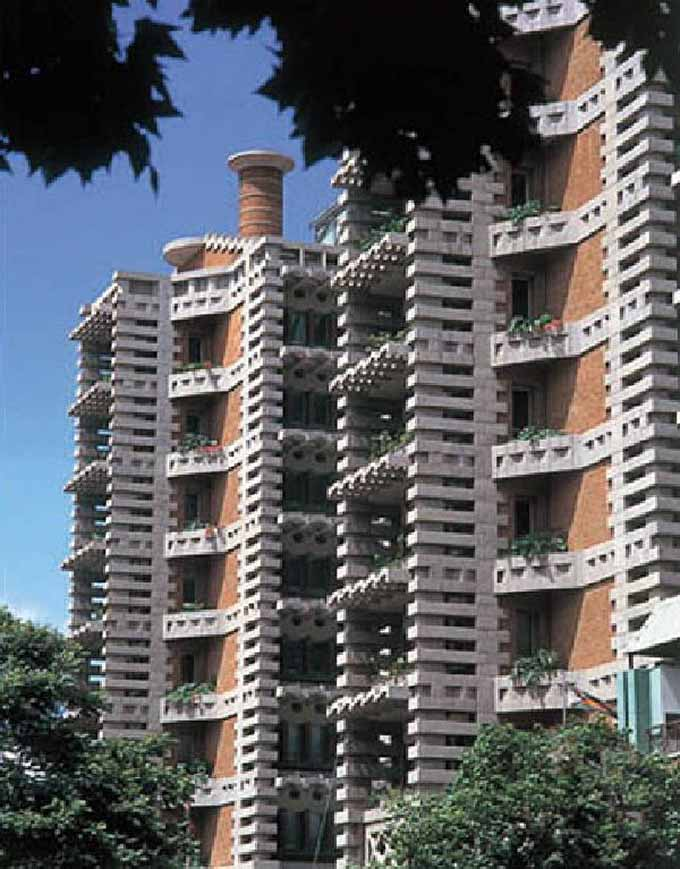
\includegraphics[width=.9
		\textwidth]{arup_building}
		\caption*{Building in Harare, Zimbabwe is modelled after termite mounds. Photo by Mike Pearce.}\label{fig:arup_building} \end{subfigure}
	\hspace*{1em}
	\begin{subfigure}
		[b]{.35
		\textwidth} \centering
		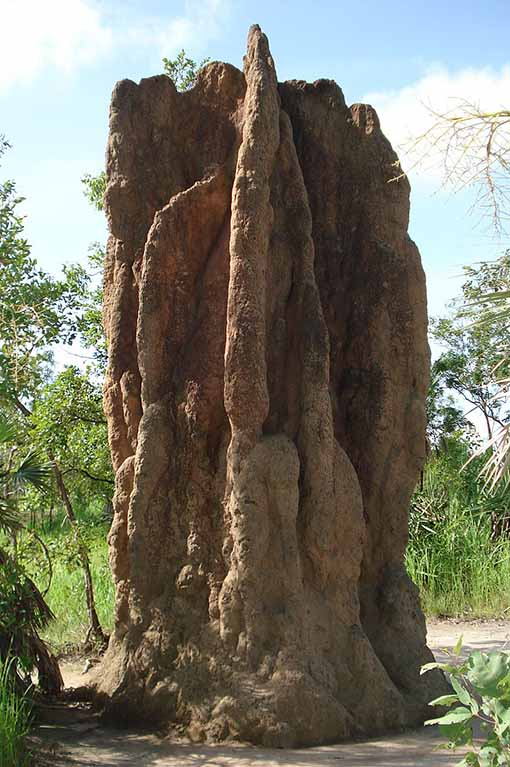
\includegraphics [width=.9
		\textwidth]{termite_cathedral}
		\caption*{Cathedral termite mound, Australia. Photo by Awoisoak Kaosiowa, 2008.}\label{fig:termite_cathedral} \end{subfigure}
	\end{sidecaption}\label{fig:termites}
\end{figure}

See \cref{fig:termites}, termites self-cooling mounds keep the temperature inside at exactly \(31^{\circ} C\), ideal for their fungus-farming; while the temperatures outside range from 2 to \(40^{\circ} C\) through the day. Such building techniques inspired architect Mike Pearce to design a shopping mall in Zimbabwe that uses a tenth of the energy used by a conventional building of the same size.

From where does termites intelligence come?
\begin{quotation}
	\small \emph{Individual termites react rather than think, but at a group level, they exhibit a kind of cognition and awareness of their surroundings. Similarly, in the brain, individual neurons do not think, but thinking arises in their connections.}\flushright{} --- Radhika Nagpal, Harvard University~\cite{margonelli:2016}.
\end{quotation}

Such collective intelligence happens in groups of just a couple of million termites. There are around 80 to 90 billion neurons in the human brain, each one of them less capable than a termite, but collectively they show still uncomparable intelligence capabilities.

\begin{figure}
	[ht!] \centering
	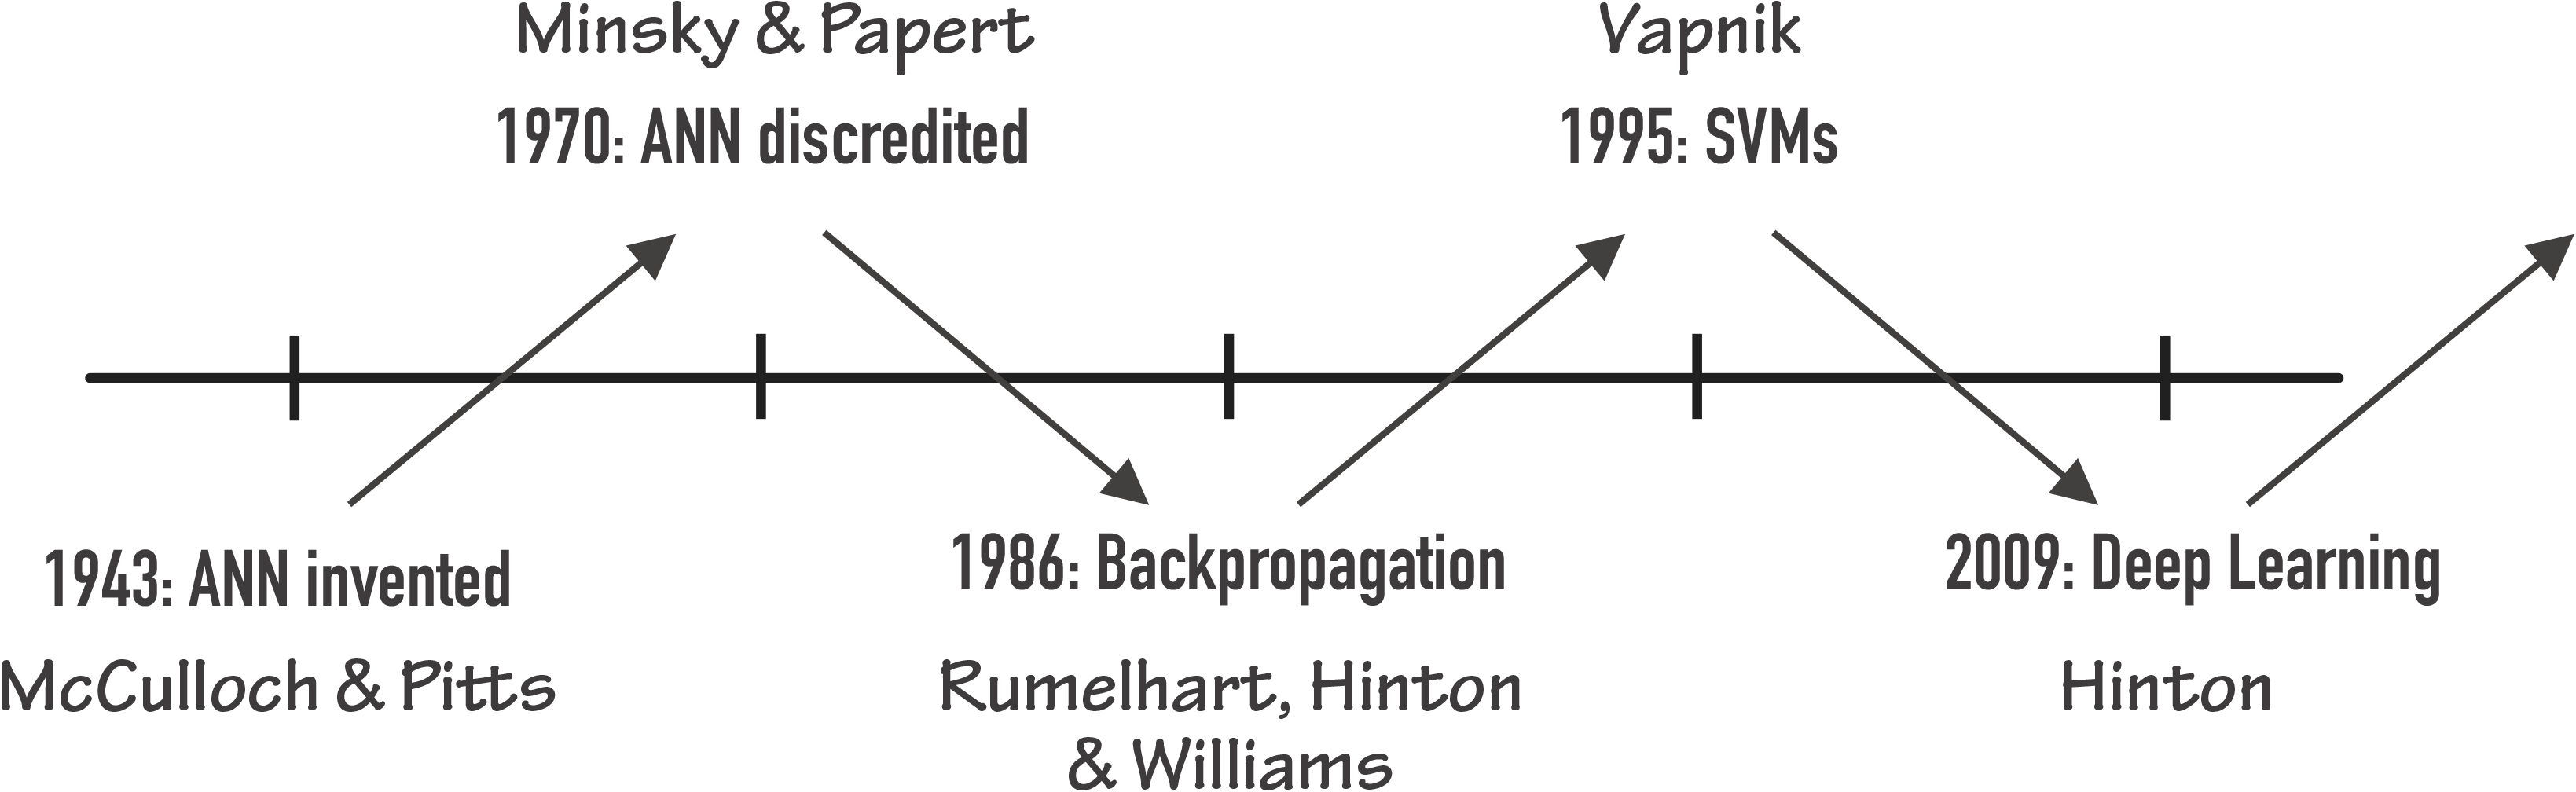
\includegraphics[width=0.8
	\textwidth]{winters}
	\caption{A brief history of connectionism. Inspired by~\citeonly{tishby:2020DeepMath}.}\label{fig:connectionism}
\end{figure}
In contrast with the symbolic approach, in neural networks, the knowledge is not explicit in symbols but implicit in the strength of the connections between the neurons. Besides, it is a very general and flexible approach since these connections can be updated algorithmically: they are algorithms that \emph{learn}: the connectionist approach is an example of what we now call Machine Learning.


\subsection{Machine Learning}
\sidefigure{lulu}{0}{Is this a cat?}

Look at the \cref{fig:lulu}. Is this a picture of a cat? How to write a program to do such a simple classification task (cat/no cat)? One could develop clever ways to use \emph{features} from the input picture and process them to make a guess. Though, it is not an easy program to design. Worse, even if one manages to program such a task, how much would it worth to accomplish a related task, to recognise a dog, for example?

For a long, this was the problem of researchers in many areas of interest of AI:\@ \acf{CV}, \acf{NLP}, Speech Recognition; much mental effort was put, with inferior results, in problems that we humans solve with ease.

The solution is an entirely different approach for building artificial intelligence: instead of building the program to do the task, build the program that outputs the program that does the task. In other words, learning algorithms use what we call ``training data'' to infer the transformations to the input that generates the desired output. It is competence without comprehension.

\subsubsection{Types of learning} Machine Learning can happen in different scenarios, which differ in the availability of training data, how training data is received, and how the test data is used to evaluate the learning. Here, we describe the most typical of them~\cite{mohri:2012}:
\begin{itemize}
	\item \textbf{Supervised learning:} The most successful scenario. The learner receives a set of labelled examples as training data and makes predictions for unseen data.
	\item \textbf{Unsupervised learning:} The learner receives unlabeled training data and makes predictions for unseen instances.
	\item \textbf{Semi-supervised learning:} The learner receives a training sample consisting of both labelled and unlabelled data and makes predictions for unseen examples. Semi-supervised learning is usual in settings where unlabeled data is easily accessible, but labelling is too costly.
	\item \textbf{Reinforcement learning:} The learner actively interacts with the environment and receives an immediate reward for her actions. The training and testing phases are intermixed.
\end{itemize}

\subsection{Deep Learning} The \(2010_s\) have been an AI Renaissance not only in academia but also in the industry. Almost all the successes are due to \acf{DL}, in particular, supervised deep learning with vast amounts of data trained in \acfp{GPU}. It was the decade of \ac{DL}.

\emph{``Deep learning algorithms seek to exploit the unknown structure in the input distribution to discover good representations, often at multiple levels, with higher-level learned features defined in terms of lower-level features~\citeauthor{bengio:2012}}''.The name is explained by one of his students~\cite{goodfellow:2016}: ``\emph{A graph showing the concepts being built on top of each other is a deep graph. Therefore the name, deep learning}''. Although it is a direct descendant of the connectionist movement, it goes beyond the neuroscientific perspective in its modern form. It is more a general principle of learning multiple levels of compositions.

The quintessential example of a deep learning model is the deep feedforward network or \acf{MLP}~\cite{russell:2010}.
\begin{figure}[hbt!]
	\begin{neuralnetwork}
		[height=4]
		\newcommand{\x}[2]{\(x_#2\)}
		\newcommand{\y}[2]{\(\hat{y}_#2\)}
		\newcommand{\hfirst}[2]{\small \(h^{(1)}_#2\)}
		\newcommand{\hsecond}[2]{\small \(h^{(2)}_#2\)} \inputlayer[count=3, bias=true, title=Input\\layer, text=\x] \hiddenlayer[count=4, bias=false, title=Hidden\\layer 1, text=\hfirst] \linklayers \hiddenlayer[count=3, bias=false, title=Hidden\\layer 2, text=\hsecond] \linklayers \outputlayer[count=2, title=Output\\layer, text=\y] \linklayers
	\end{neuralnetwork}
	\end{figure}
\begin{definition}
	Let,
	\begin{itemize}
		[leftmargin=1.5cm]
		\item [\(\vx\)] be the input vector \(\{\vx_1, \ldots, \vx_m\}\)
		\item[\(k\)] be the layer index, such that \(k \in [1,l] \),
		\item[\(d_k\)] is the number of elements in the hidden layer \({(k)}\),
		\item[\(\mW^{(k)}_{i,j}\)] be the matrix of weights in the \(k\)-th layer, where \( i \in [0,d_{k-1}], j \in [1, d_k] \text{ and }\mW^{(k)}_{0,:}\) are the biases
		\item[\(\sigma~\)] be a non-linear function,
	\end{itemize}
	a \textbf{\acfp{MLP}} is a neural network where the input is defined by:
	\begin{align}
		h^{(0)}= 1^\frown \vx,
	\end{align}
	a hidden layer is defined by:
	\begin{align}
		h^{(k)}&=\sigma^{(k)}(\mW^{(k)~\top} h^{(k-1)}).
	\end{align}
	The output is defined by:
	\begin{align}
		\hat{y}&=h^{(l)}.
	\end{align}
\end{definition}


Deep Learning is usually associated with \acfp{DNN}, but the network architecture is only one of its components:
\begin{enumerate}
	\item DNN architecture
	\item \acf{SGD} --- the optimiser
	\item Dataset
	\item Loss function
\end{enumerate}

The architecture is not the sole component essential to current Deep Learning success. The \ac{SGD} plays a crucial role, and so does the usage of large datasets.

A known problem, though, is that DNNs are prone to overfitting (\cref{sec:bias-variance}). ~\citeauthor{zhang:2016} shows that state-of-the-art convolutional deep neural networks can easily fit a random labelling of training data.
